%--------------------------------------
% Create title frame
\titleframe

%--------------------------------------
% Table of contents
\begin{frame}{Overview}
  \setbeamertemplate{section in toc}[sections numbered]
  \tableofcontents[hideallsubsections]
\end{frame}


% What will we learn slide
\begin{frame}{What will we learn today?}
    \small
    Mostly from Chapter 2 of Ned Mohan's book:

    \begin{center}
        Mohan, Ned. Electric power systems: a first course. John Wiley \& Sons, 2012.
    \end{center}

    \begin{itemize}
        \item 3-phase systems
        \item Power transfer between AC systems
        \item Per unit normalization
    \end{itemize}
    You will be able to do exercises 2.1, 2.2, 2.4, 2.5, 2.9, 2.11, 2.12, 2.14, 2.16, 2.17, 2.18, 2.19 and 2.20 from the Ned Mohan's book.
\end{frame}



\section{Three-phase systems (reminder)}
% Three-phase system slide
\begin{frame}{Three-phase system }
\begin{columns}
    \begin{column}{0.7\textwidth}
    \begin{figure}
        \centering
        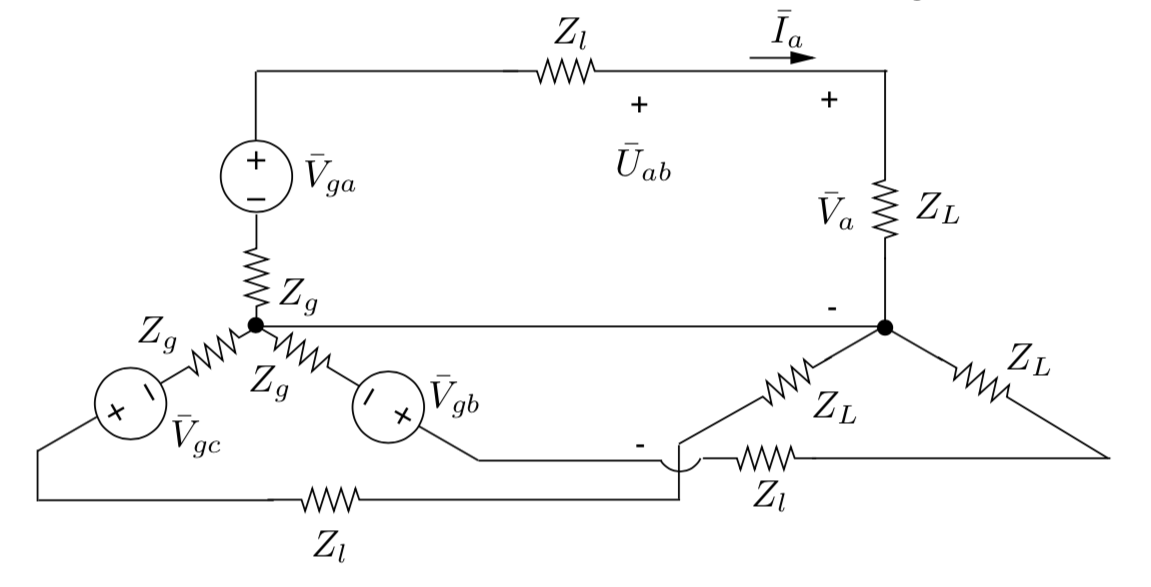
\includegraphics[width=0.99\textwidth]{images/three-phase-system.png}
        \caption{Generation -> transmission -> load}
    \end{figure}
    \end{column}
    \begin{column}{0.3\textwidth}
    Here the load is connected as a \textit{star}. A neutral point is present. The neutral conductor is not necessarily implemented.
    \end{column}
\end{columns}
\end{frame}

% Voltage sources slide
\begin{frame}{By design the voltage sources are shifted by 120°}
    \begin{columns}
    \begin{column}{0.4\textwidth}
        \begin{align*}
        \bar{V}_{ga} &= V e^{j\phi_u} \\
        \bar{V}_{gb} &= V e^{j(\phi_u - 2 \pi / 3)} = \bar{V}_{ga} e^{-j 2 \pi / 3} \\
        \bar{V}_{gc} &= V e^{j(\phi_u - 4 \pi / 3)} = \bar{V}_{ga} e^{-j 4 \pi / 3}
        \end{align*}
    \end{column}
    \begin{column}{0.6\textwidth}
        \begin{figure}
            \centering
            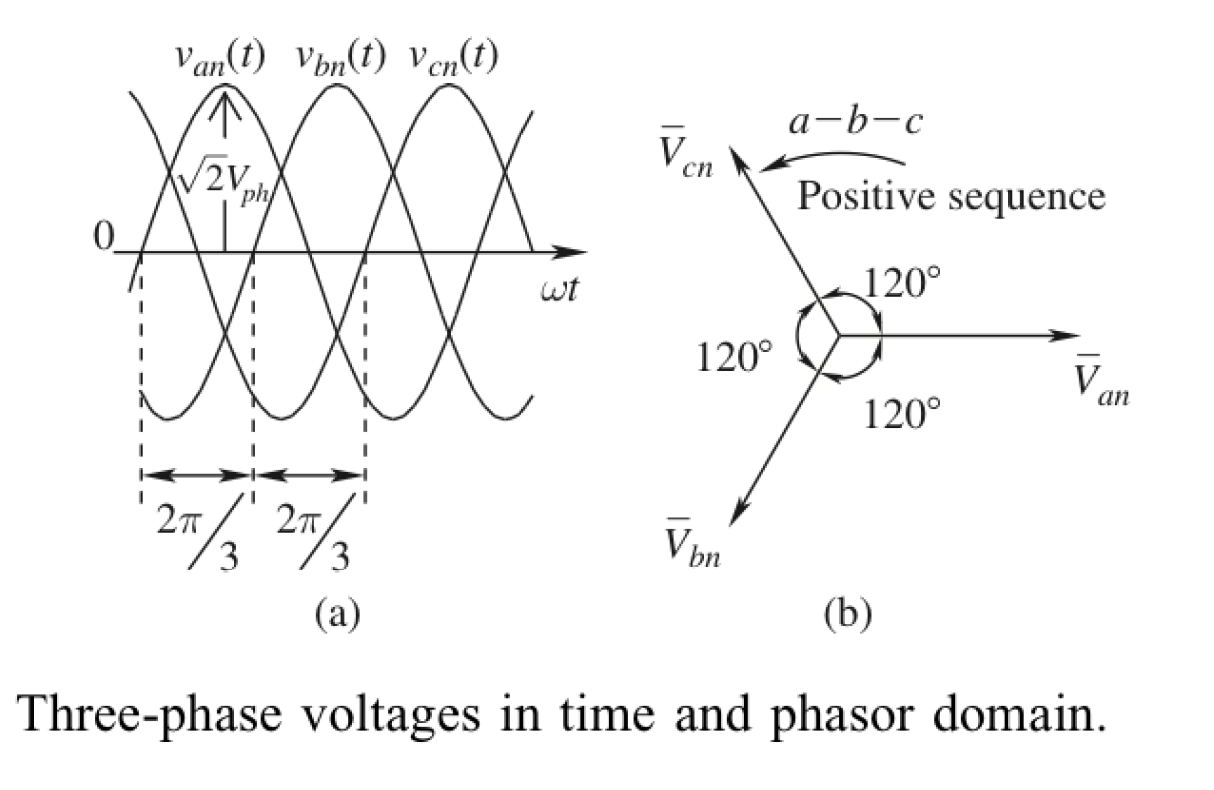
\includegraphics[width=0.99\textwidth]{images/3ph_time_vs_phasor.PNG}
        \end{figure}
    \end{column}
\end{columns}

\end{frame}

% Phase voltage vs line to line voltage slide
\begin{frame}{Phase voltage vs. line to line voltage}

    \begin{columns}
    \begin{column}{0.5\textwidth}
        These voltages represent the \textbf{phase voltages}. If we now look at the \textbf{line to line voltages}:
        $$
        \bar{U}_{ab} = \bar{V}_{ga} - \bar{V}_{gb} = \sqrt{3} \bar{V}_{ga} e^{j\pi / 6}
        $$
        and similarly for $\bar{U}_{bc}$ and $\bar{U}_{ca}$.
    \end{column}
    \begin{column}{0.5\textwidth}
        \begin{figure}
        \centering
        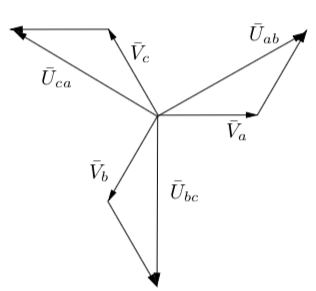
\includegraphics[width=0.6\textwidth]{images/line_vs_phase_voltage_diagram.png}
        \caption{Line vs. phase voltages}
        \end{figure}
    \end{column}
\end{columns}

\textit{Example:} My house is fed by a 400V three-phase system. This means the line voltages are 400V (rms), and thus phase voltages are 230V (approximately). Typically, the phase voltages are distributed independently in the house, each with the neutral.

\end{frame}

% Total power slide
\begin{frame}{Total power}
    The total complex power transmitted to the load is
    $$
    S = \sum_{k \in \{a, b, c\}} \bar{V}_{gk} \bar{I}^*_{k}
    $$
    Hence in a balanced system the total active power to the load is $3VI \cos \phi$, with 3 or 4 wires (instead of 2 in a single-phase system).
\end{frame}


% Comments slide
\begin{frame}{Comments}
    \begin{itemize}
        \item In every phase there is a current flowing. In a balanced system, currents are phase shifted by 120° and sum to zero. Thus the neutral can in theory be removed. This is done in some portions of the global system (typically at high voltage), where neutral points are grounded.
        \item Some loads can also be connected in "delta", hence the neutral is not accessible.
        \item Finally, in unbalanced systems, currents are dictated by the impedances seen in the different phases. There is no perfectly known relation, a priori.
    \end{itemize}
\end{frame}

% Exercise slide
\section{Neutral break exercise}
\begin{frame}{Neutral break: problem statement}
    Consider a 3-phase Y-connected resistive circuit with unbalanced resistors in the phases. In normal operation there is a neutral wire. Then the neutral breaks.
    \begin{itemize}
        \item Compute in both cases the voltages across the resistors, the currents and the consumed powers.
        \item What can you observe?
    \end{itemize}
    \textbf{Remark}: In the next slides, the phasor notation is omitted, but all voltages and currents should be understood as phasors.
\end{frame}

% Case 1: Neutral Connected slide
\begin{frame}{Case 1: Neutral Connected}
    \textbf{Assumptions:}
    \begin{itemize}
        \item 3-phase balanced voltage supply: $V_{ab} = V_{bc} = V_{ca} = V_L$ (line-to-line voltage)
        \item Phase voltages (line-to-neutral) are given by $V_{an} = V_{bn} = V_{cn} = \frac{V_L}{\sqrt{3}}$, and the angle between them is $120^\circ$.
        \item Unbalanced resistances: $R_a$, $R_b$, $R_c$ (different resistances in each phase).
    \end{itemize}
\end{frame}
\begin{frame}{Voltages and currents}
    \textbf{Voltages:} In normal operation, with the neutral connected, each resistor has its corresponding phase voltage across it:
    $$V_{R_a} = V_{an}, \quad V_{R_b} = V_{bn}, \quad V_{R_c} = V_{cn}$$
    \textbf{Currents:} The current in each phase is given by Ohm's law:
    $$I_a = \frac{V_{an}}{R_a}, \quad I_b = \frac{V_{bn}}{R_b}, \quad I_c = \frac{V_{cn}}{R_c}$$
    The neutral current, $I_n$, is the sum of the phase currents:
    $$I_n = I_a + I_b + I_c$$
    Due to the unbalanced resistances, $I_n$ will not be zero.
\end{frame}

% Powers slide
\begin{frame}{Powers}
    The power consumed in each phase is:
    $$P_a = V_{an} I_a = \frac{V_{an}^2}{R_a}, \quad P_b = \frac{V_{bn}^2}{R_b}, \quad P_c = \frac{V_{cn}^2}{R_c}$$
    Total power consumed:
    $$P_{\text{total}} = P_a + P_b + P_c$$
\end{frame}

% Case 2: Neutral Broken slide
\begin{frame}{Case 2: Neutral Broken}
    When the neutral breaks, the three resistors form a system without a direct connection to the neutral point. The current through each resistor still needs to sum to zero because the current has no return path through the neutral. This changes the voltage distribution across the resistors.
\end{frame}

% Voltages: slide
\begin{frame}{Voltages and currents}
    Here, $ V_{nN'} $ is an unknown voltage offset at the floating point $ N' $ (the shifted neutral). Using KCL, you solve for this voltage by ensuring the sum of the currents at $ N' $ is zero:
    $$
    \frac{V_{aN'}}{R_a} + \frac{V_{bN'}}{R_b} + \frac{V_{cN'}}{R_c} = 0
    $$
    Solving this system gives you the new voltages across the resistors.

    \begin{itemize}
        \item The currents in each phase are then given by:
        $$
        I_a = \frac{V_{aN'}}{R_a}, \quad I_b = \frac{V_{bN'}}{R_b}, \quad I_c = \frac{V_{cN'}}{R_c}
        $$
        \item Since the neutral is broken, the sum of these currents must equal zero:
        $$
        I_a + I_b + I_c = 0
        $$
    \end{itemize}
\end{frame}

% Powers: slide
\begin{frame}{Powers}
    \begin{itemize}
        \item The power consumed in each phase is:
        $$
        P_a = V_{aN'} I_a = \frac{(V_{aN'})^2}{R_a}, \quad P_b = \frac{(V_{bN'})^2}{R_b}, \quad P_c = \frac{(V_{cN'})^2}{R_c}
        $$
        \item Total power consumed:
        $$
        P_{\text{total}} = P_a + P_b + P_c
        $$
    \end{itemize}
\end{frame}

% Observations: slide
\begin{frame}{Observations}
    \begin{itemize}
        \item When the neutral is connected, the voltages across the resistors are straightforwardly determined by the phase-to-neutral voltages.
        \item When the neutral is broken, the voltage distribution becomes more complex, and the voltages across the resistors are no longer the same as the phase-to-neutral voltages. The total current in the system remains zero, and the power distribution can also change depending on the values of the resistors.
    \end{itemize}
    \href{https://colab.research.google.com/drive/1pXH21c8g9Hv3h94pb81OtuFVQfauG63T?usp=sharing}{A numerical example here.}
\end{frame}

% Useful formulas slide
\begin{frame}{Useful formulas: from star to delta connection (and back)}
    \begin{figure}
        \centering
        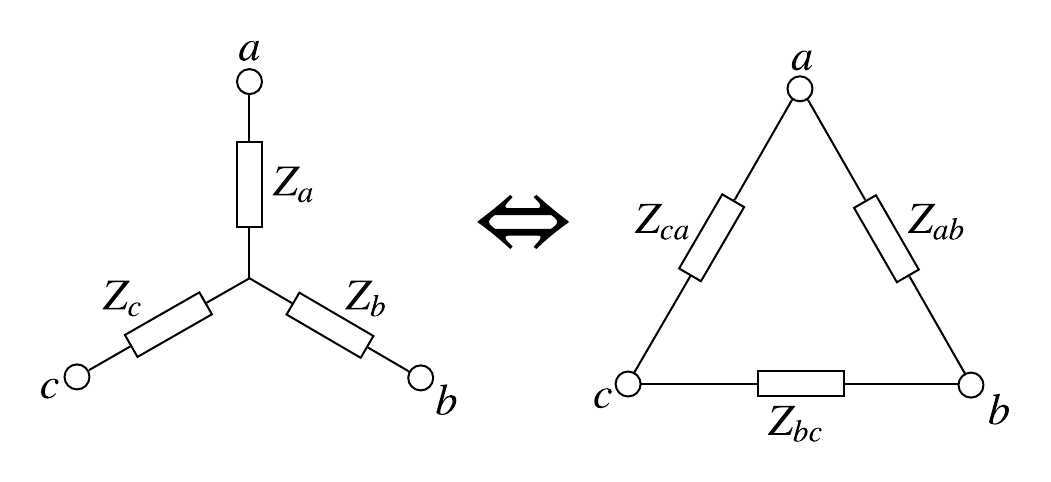
\includegraphics[width=0.5\textwidth]{images/star_delta.png}
    \end{figure}
    \begin{columns}
        \begin{column}{0.5\textwidth}
            $$ \begin{aligned}
            Z_a &= \frac{Z_{ab}Z_{ca}}{Z_{ab} + Z_{bc} + Z_{ca}} \\
            Z_b &= \frac{Z_{bc}Z_{ab}}{Z_{ab} + Z_{bc} + Z_{ca}} \\
            Z_c &= \frac{Z_{ca}Z_{bc}}{Z_{ab} + Z_{bc} + Z_{ca}}
            \end{aligned}$$
        \end{column}
        \begin{column}{0.5\textwidth}
            $$ \begin{aligned}
            Z_{ab} &= \frac{Z_{a}Z_{b}+Z_{b}Z_{c}+Z_{c}Z_{a}}{Z_{c}} \\
            Z_{bc} &= \frac{Z_{a}Z_{b}+Z_{b}Z_{c}+Z_{c}Z_{a}}{Z_{a}} \\
            Z_{ca} &= \frac{Z_{a}Z_{b}+Z_{b}Z_{c}+Z_{c}Z_{a}}{Z_{b}}
            \end{aligned}$$
        \end{column}
    \end{columns}
    What happens in a balanced system?
\end{frame}

% Per-phase analysis slide
\section{Per-phase analysis}
\begin{frame}[allowframebreaks]{Per-phase analysis}
    In a \textbf{balanced} system, analyses can be simplified by representing only one phase.
    
    This is straightforward if there are no couplings between phases.
    \begin{figure}
        \centering
        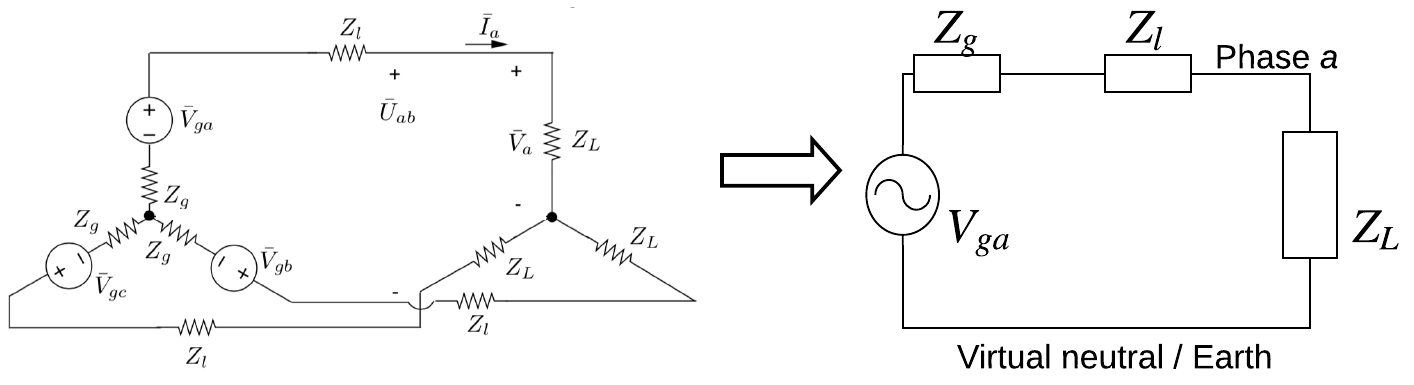
\includegraphics[width=0.8\textwidth]{images/per-phase.png}
    \end{figure}
    In case there is a coupling, and that for instance the voltage drop $\bar{V}_{aA}$ along a line presenting an impedance $Z_{self}$ traversed by a current $\bar{I}_{a}$ is also function of the currents in the other phases:
$$\bar{V}_{aA} = Z_{self} \bar{I}_{a} + Z_{mutual} \bar{I}_{b} + Z_{mutual} \bar{I}_{c}$$
then the per-phase equivalent impedance (for phase $a$) is $$Z_{aA} = Z_{self} - Z_{mutual}$$
since $\bar{I}_{a} + \bar{I}_{b} + \bar{I}_{c} = 0$
\end{frame}

\begin{frame}{One-line diagram}
\begin{figure}
        \centering
        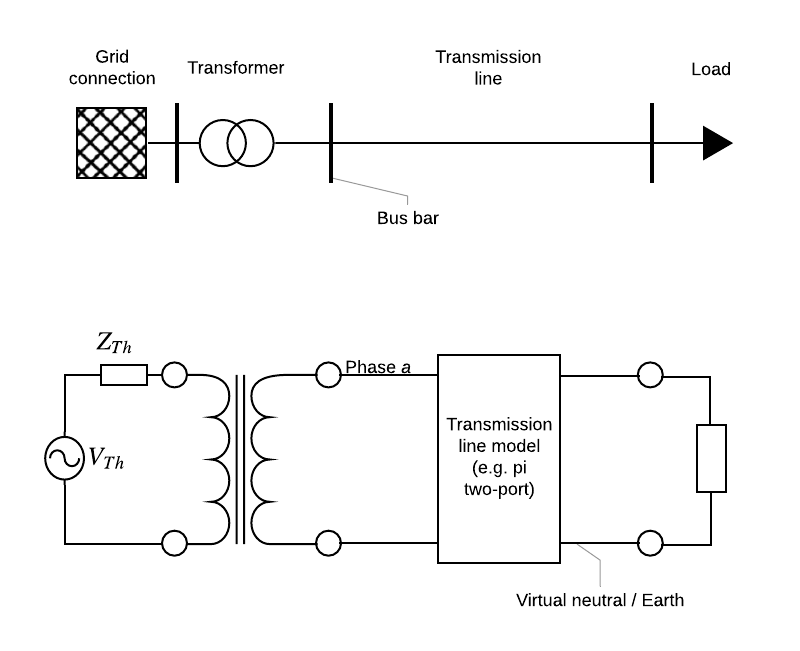
\includegraphics[width=0.6\textwidth]{images/one-line.png}
    \end{figure}
\end{frame}

\section{Power transfer between AC systems}
% Power transfer between AC systems slide
\begin{frame}[allowframebreaks]{Power transfer between AC systems}
    \begin{columns}
        \begin{column}{0.5\textwidth}
            Consider the following simple system. We have $\bar{I} = \frac{\bar{V}_s-\bar{V}_r}{jX}$
        \end{column}
        \begin{column}{0.5\textwidth}
            \begin{figure}
                \centering
                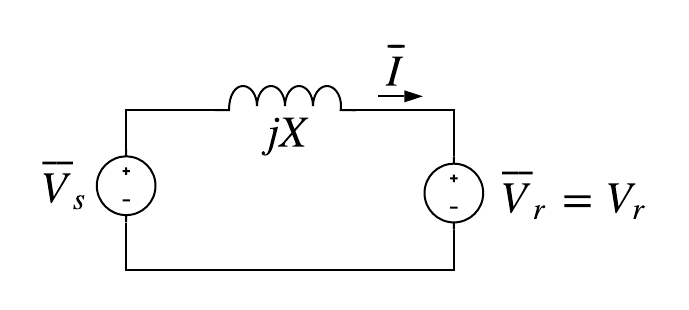
\includegraphics[width=\textwidth]{images/power-transfer_AC.png}
            \end{figure}
        \end{column}
    \end{columns}
    Let $\delta$ be the angle between $\bar{V}_r$ and $\bar{V}_s$, then
    $$
    \begin{aligned}
    S_r &= \bar{V}_r\bar{I}^* = V_r \left(\frac{V_s \angle -\delta - V_r}{-jX}\right) \\
         &= \frac{V_s V_r \sin \delta }{X} +j \frac{V_s V_r \cos \delta - V^2_r}{X}
    \end{aligned}
    $$
    \textbf{Let's remember two things:}
    \begin{itemize}
        \item The \textbf{active} power is highly sensitive to \textbf{$\delta$}
        \item The \textbf{reactive} power acts on the \textbf{voltage magnitude} (look at what happens for $\delta=0$)
    \end{itemize}

    See \href{https://colab.research.google.com/drive/1wrJYI082Y6qE6TyaT5a7eWO1lB0CCWiu?usp=sharing}{\underline{a demo}}.
\end{frame}


% Per-unit normalization slide
\section{Per-unit normalization}

% Per-unit values slide
\begin{frame}{Per-unit values}
    Per-unit values are the ratio between the actual value and the base value.
    $$
    \text{Value}_{pu} = \frac{\text{Actual value}}{\text{Base value}}
    $$
    It is useful in electrical power systems for two reasons:
    \begin{itemize}
        \item The parameters of rotating machines and transformers provided by the manufacturers are often given in pu.
        \item In a transformer, the impedance (in ohm) changes according to the square of the voltage ratio. If we express the impedance in pu, the value is invariant from one side of the transformer to the other.
    \end{itemize}
    In an electric network, a single base power is sufficient for the whole system, but for a system with transformers, one base voltage per voltage level is preferable.
\end{frame}

% Example slide
\begin{frame}[allowframebreaks]{Example}
    It is \textbf{known} that the internal reactance of a synchronous machine lies typically in the range $[1.5, 2.5] \text{ pu}$ (on the machine base)! 
     
    A machine with the characteristics $(20 \text{ kV}, 300 \text{ MVA})$ has a reactance of $2.667 \ \Omega$.\\ Is this a normal value?
    \begin{itemize}
        \item (Here we do not need a base value for time)
        \item The base impedance is $Z_B = 20^2/300 = 1.333 \ \Omega$
        \item Hence the value of the reactance in per unit is $2.667/1.333 = 2 \ pu$
        \item This is a quite normal value!
    \end{itemize}
    Same question for a machine with the characteristics $(15 \text{ kV}, 30 \text{ MVA})$
    \begin{itemize}
        \item The base impedance is now $Z_B=15^2/30 = 7.5 \ \Omega$
        \item The value of the reactance in per unit is $2.667/7.5 = 0.356 \ pu$
        \item Hence an abnormal small value!
    \end{itemize}
\end{frame}

% Per unit in three-phase systems slide
\begin{frame}{Per unit in three-phase systems}
    Let the base power $S_B$ be the three-phase power, and $U_b=\sqrt{3}V_B$ be the line to line voltage base.

    The (single-phase) base current is $$I_B = \frac{S_B}{3V_B} = \frac{S_B}{\sqrt{3}U_B}$$

    The base impedance is $$Z_B = \frac{V_B}{I_B} = \frac{3V^2_B}{S_B} = \frac{U_B^2}{S_B}$$

    In a single phase equivalent representation, the power values in per unit can be multiplied by $S_b$ to get the total three-phase power.
\end{frame}
  